\chapter{Training Configuration}
\label{chap:train}

\section{Hardware and Software Environment}

All experiments were conducted on Google Colab using a single NVIDIA T4 GPU (16~GB VRAM).
The software stack is PyTorch~2.0 with CUDA~11.8, \texttt{nibabel} for NIfTI I/O, and
\texttt{scipy} for distance-transform computations used inside the HD95 metric. Automatic Mixed Precision (AMP) was
enabled via \texttt{torch.cuda.amp} to reduce VRAM consumption and accelerate forward passes
by approximately $1.4\times$. Gradient clipping (maximum $\ell_2$ norm of~$1.0$) was applied
at each backward pass to prevent exploding gradients during early training.

\section{Hyperparameters}

Table~\ref{tab:hyperparams} lists the fixed hyperparameters for Run~017, the final and best
configuration.

\begin{table}[h!]
\centering
\caption{Training hyperparameters for Run~017.}
\label{tab:hyperparams}
\begin{tabular}{ll}
\toprule
\textbf{Hyperparameter} & \textbf{Value} \\
\midrule
Optimiser               & Adam ($\beta_1 = 0.9$, $\beta_2 = 0.999$) \\
Initial learning rate   & $1 \times 10^{-3}$ \\
LR schedule             & \texttt{CosineAnnealingLR} \\
$T_{\max}$ (cosine period) & 60 epochs \\
$\eta_{\min}$           & $1 \times 10^{-6}$ \\
Batch size              & 8 \\
Input image size        & $256 \times 256$ \\
Number of epochs        & 60 \\
Early stopping patience & 10 (not triggered) \\
Gradient clip norm      & 1.0 \\
Mixed precision (AMP)   & Enabled \\
Training volumes        & 42 (3{,}785 slices) \\
Validation volumes      & 8 (754 slices) \\
Training time           & $\approx 79.6$~minutes \\
\bottomrule
\end{tabular}
\end{table}

\section{Learning Rate Schedule}

\texttt{CosineAnnealingLR} decays the learning rate smoothly from $\eta_{\max} = 10^{-3}$ to
$\eta_{\min} = 10^{-6}$ over $T_{\max} = 60$ epochs following:

\begin{equation}
  \eta_t = \eta_{\min} + \frac{1}{2}\left(\eta_{\max} - \eta_{\min}\right)
  \left(1 + \cos\!\frac{\pi t}{T_{\max}}\right)
\end{equation}

Figure~\ref{fig:lr_schedule} compares cosine annealing with a step-based schedule at equivalent
parameter budget. The cosine schedule avoids the abrupt drops of step decay and maintains a
higher learning rate through mid-training, allowing continued feature refinement before the
final slow convergence phase.

\begin{figure}[h!]
\centering
\begin{minipage}{0.85\textwidth}
  \centering
  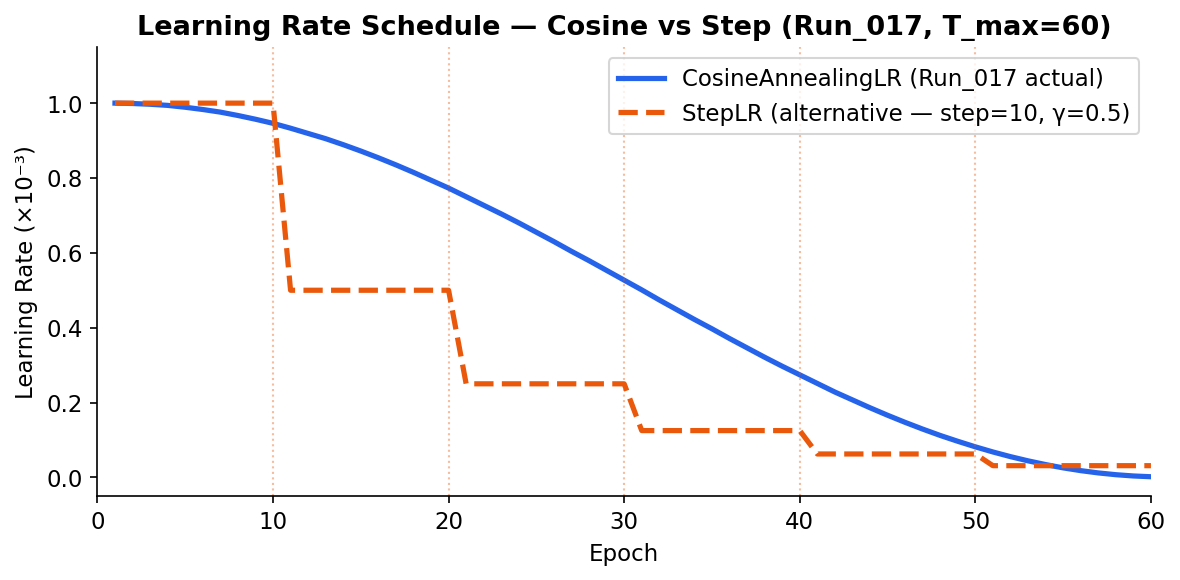
\includegraphics[width=\textwidth]{figures/fig_lr_schedule}
  \caption{CosineAnnealingLR versus a step-based schedule over 60 epochs. The cosine schedule
  (blue) decays smoothly; the step schedule (orange) drops abruptly at fixed milestones.
  Values are from Run~017's actual training run.}
  \label{fig:lr_schedule}
\end{minipage}
\end{figure}

\FloatBarrier

\section{Training Curves}

Figure~\ref{fig:training_curves} shows the per-epoch training and validation loss, together
with the validation Dice, over all 60 epochs of Run~017.

\begin{figure}[h!]
\centering
\begin{minipage}{0.90\textwidth}
  \centering
  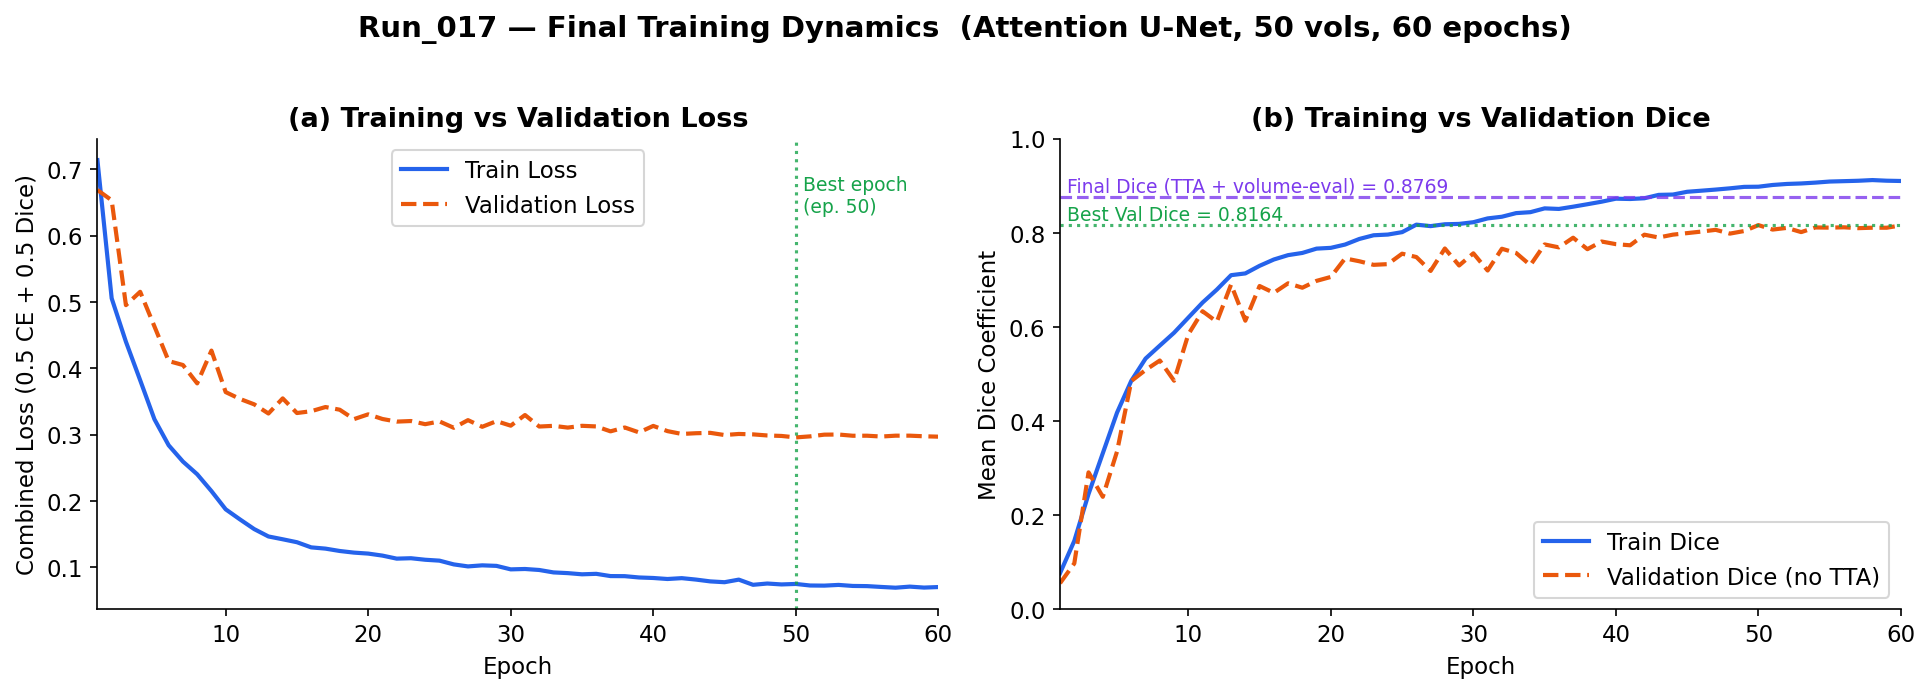
\includegraphics[width=\textwidth]{figures/fig_training_curves}
  \caption{Run~017 training curves. Left: training loss (blue) and validation loss (orange)
  over 60 epochs. Right: validation Dice (per-volume) over 60 epochs. The model converged
  smoothly with no signs of overfitting; the best validation Dice of 0.8164 (without TTA)
  was recorded at epoch~50.}
  \label{fig:training_curves}
\end{minipage}
\end{figure}

\FloatBarrier

What the curves show is encouraging. Training loss drops steeply in the first 15 epochs, then
continues falling gradually to a final value of $0.0702$. Validation loss tracks closely
throughout --- final value $0.2970$ --- with no divergence that would indicate overfitting. The
gap between training and validation loss is partly expected: training loss is computed on raw
logits with the combined loss, while validation Dice is computed on softmax probabilities for
the 13 foreground classes only.

The best checkpoint (epoch~50, val Dice $= 0.8164$ without TTA) was saved and used for all
subsequent evaluation runs. Epochs~51--60 show marginal loss improvement but no gain in
validation Dice, consistent with the cosine schedule driving the learning rate below $5 \times
10^{-5}$ after epoch~50. Early stopping (patience~10) did not trigger.

\section{Training Pseudocode}

\begin{verbatim}
for epoch in range(NUM_EPOCHS):
    model.train()
    for batch in train_loader:
        optimizer.zero_grad()
        with autocast():
            logits = model(batch['image'])
            loss = 0.5 * ce_loss(logits, batch['mask'])
                 + 0.5 * dice_loss(logits, batch['mask'])
        scaler.scale(loss).backward()
        scaler.unscale_(optimizer)
        clip_grad_norm_(model.parameters(), max_norm=1.0)
        scaler.step(optimizer)
        scaler.update()
    scheduler.step()

    model.eval()
    val_dice = per_volume_dice(model, val_loader)
    if val_dice > best_dice:
        best_dice = val_dice
        torch.save(model.state_dict(), 'best_model.pth')
\end{verbatim}
